\pagebreak

\section{Introduction}
\label{sec:introduction}

\paragraph{}The very fundamental concept that characterizes an amplifier is its ability to convert a low strength input signal into one of higher strength. In our daily lives, there are multiple applications of this type of devices. What perhaps is the most common form we can find it is in audio components, more specifically, in speakers, which the sound enters with a lower level and exits with a higher one. Besides the already mentioned use of amplifiers in speakers, the truth is that there are many other interesting possible applications. Among them, we have multiple examples such as alarms, sensors and protections systems.

\paragraph{}
In Section~\ref{sec:theoretical}, a theoretical introduction is made in order to contextualize all the main principles that sustain our construction and analysis of the circuit. A theoretical Audio Amplifier circuit is built and carefully analysed in Section~\ref{analysis}, where the results are obtained in GNU Octave. Also, in Section~\ref{sec:simulation}, the Audio Amplifier circuit is analysed by simulation through the use of NGSpice to simulate the real electric circuit behaviour. The results of the simulation of Section~\ref{sec:simulation} are then compared to the theoretical results obtained in Section~\ref{analysis} and the comparative results are expressed in Section~\ref{error}. The figure of merit, calculated according to the components used to build the simulation circuit, can also be found in Section~\ref{error}. The conclusions of this study are outlined in the final part of the report, in Section~\ref{sec:conclusion}.

\begin{figure}[H] \centering
	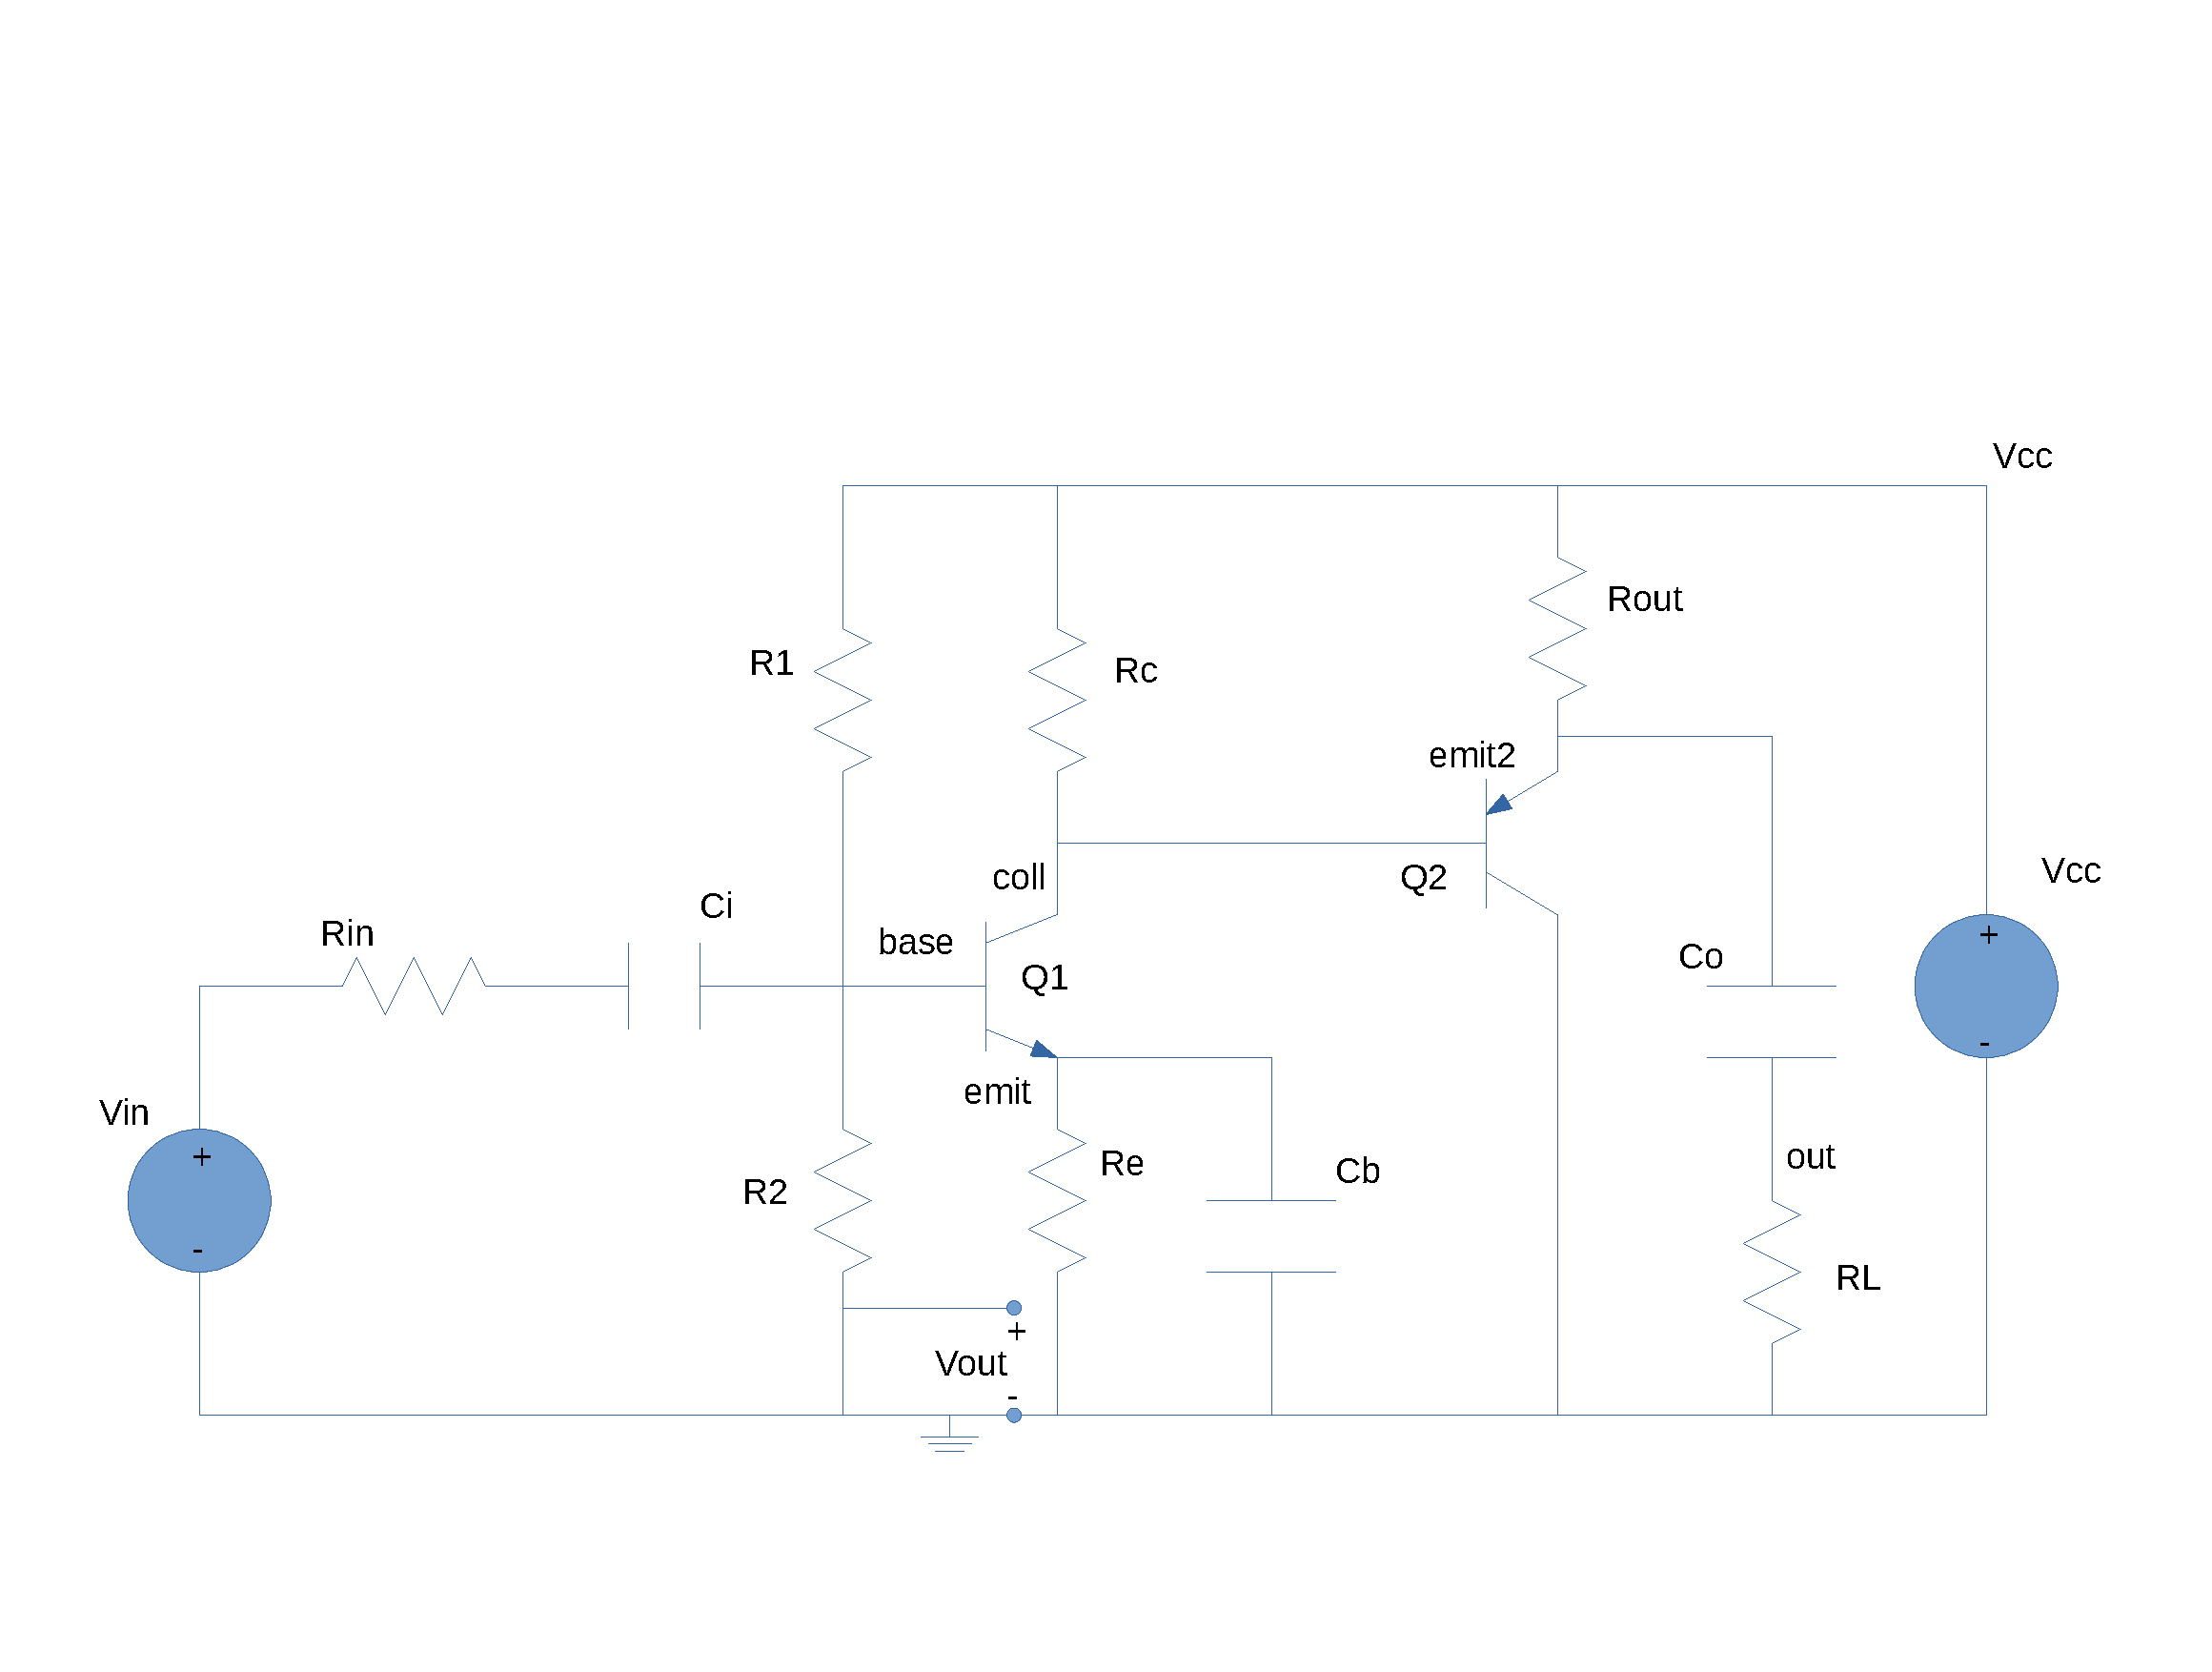
\includegraphics[width=0.7\linewidth]{circuit.pdf}
	\caption{Fourth laboratory circuit.}
	\label{fig:circuit}
\end{figure}
